\documentclass{sigchi}

% Use this section to set the ACM copyright statement (e.g. for
% preprints).  Consult the conference website for the camera-ready
% copyright statement.

% Copyright
\CopyrightYear{2018}
%\setcopyright{acmcopyright}
\setcopyright{acmlicensed}
%\setcopyright{rightsretained}
%\setcopyright{usgov}
%\setcopyright{usgovmixed}
%\setcopyright{cagov}
%\setcopyright{cagovmixed}
% DOI
\doi{http://dx.doi.org/10.475/123_4}
% ISBN
\isbn{123-4567-24-567/08/06}
%Conference
\conferenceinfo{CHI'16,}{May 07--12, 2016, San Jose, CA, USA}
%Price
\acmPrice{\$15.00}

% Use this command to override the default ACM copyright statement
% (e.g. for preprints).  Consult the conference website for the
% camera-ready copyright statement.


%% HOW TO OVERRIDE THE DEFAULT COPYRIGHT STRIP --
%% Please note you need to make sure the copy for your specific
%% license is used here!
% \toappear{
% Permission to make digital or hard copies of all or part of this work
% for personal or classroom use is granted without fee provided that
% copies are not made or distributed for profit or commercial advantage
% and that copies bear this notice and the full citation on the first
% page. Copyrights for components of this work owned by others than ACM
% must be honored. Abstracting with credit is permitted. To copy
% otherwise, or republish, to post on servers or to redistribute to
% lists, requires prior specific permission and/or a fee. Request
% permissions from \href{mailto:Permissions@acm.org}{Permissions@acm.org}. \\
% \emph{CHI '16},  May 07--12, 2016, San Jose, CA, USA \\
% ACM xxx-x-xxxx-xxxx-x/xx/xx\ldots \$15.00 \\
% DOI: \url{http://dx.doi.org/xx.xxxx/xxxxxxx.xxxxxxx}
% }

% Arabic page numbers for submission.  Remove this line to eliminate
% page numbers for the camera ready copy
% \pagenumbering{arabic}

% Load basic packages
\usepackage{balance}       % to better equalize the last page
\usepackage{graphics}      % for EPS, load graphicx instead 
\usepackage[T1]{fontenc}   % for umlauts and other diaeresis
\usepackage{txfonts}
\usepackage{mathptmx}
\usepackage[pdflang={en-US},pdftex]{hyperref}
\usepackage{color}
\usepackage{booktabs}
\usepackage{textcomp}

% Some optional stuff you might like/need.
\usepackage{microtype}        % Improved Tracking and Kerning
% \usepackage[all]{hypcap}    % Fixes bug in hyperref caption linking
\usepackage{ccicons}          % Cite your images correctly!
% \usepackage[utf8]{inputenc} % for a UTF8 editor only
\usepackage{float}

% If you want to use todo notes, marginpars etc. during creation of
% your draft document, you have to enable the "chi_draft" option for
% the document class. To do this, change the very first line to:
% "\documentclass[chi_draft]{sigchi}". You can then place todo notes
% by using the "\todo{...}"  command. Make sure to disable the draft
% option again before submitting your final document.
\usepackage{todonotes}

% Paper metadata (use plain text, for PDF inclusion and later
% re-using, if desired).  Use \emtpyauthor when submitting for review
% so you remain anonymous.
\def\plaintitle{}
\def\plainauthor{First Author, Second Author, Third Author,
  Fourth Author, Fifth Author, Sixth Author}
\def\emptyauthor{}
\def\plainkeywords{Authors' choice; of terms; separated; by
  semicolons; include commas, within terms only; required.}
\def\plaingeneralterms{Documentation, Standardization}

% llt: Define a global style for URLs, rather that the default one
\makeatletter
\def\url@leostyle{%
  \@ifundefined{selectfont}{
    \def\UrlFont{\sf}
  }{
    \def\UrlFont{\small\bf\ttfamily}
  }}
\makeatother
\urlstyle{leo}

% To make various LaTeX processors do the right thing with page size.
\def\pprw{8.5in}
\def\pprh{11in}
\special{papersize=\pprw,\pprh}
\setlength{\paperwidth}{\pprw}
\setlength{\paperheight}{\pprh}
\setlength{\pdfpagewidth}{\pprw}
\setlength{\pdfpageheight}{\pprh}

% Make sure hyperref comes last of your loaded packages, to give it a
% fighting chance of not being over-written, since its job is to
% redefine many LaTeX commands.
\definecolor{linkColor}{RGB}{6,125,233}
\hypersetup{%
  pdftitle={\plaintitle},
% Use \plainauthor for final version.
%  pdfauthor={\plainauthor},
  pdfauthor={\emptyauthor},
  pdfkeywords={\plainkeywords},
  pdfdisplaydoctitle=true, % For Accessibility
  bookmarksnumbered,
  pdfstartview={FitH},
  colorlinks,
  citecolor=black,
  filecolor=black,
  linkcolor=black,
  urlcolor=linkColor,
  breaklinks=true,
  hypertexnames=false
}

% create a shortcut to typeset table headings
% \newcommand\tabhead[1]{\small\textbf{#1}}

% End of preamble. Here it comes the document.
\begin{document}

\title{Misaligned Expectations: \\ Uncovering Different Aims in Universities and Industry}

\numberofauthors{2}
\author{%
  \alignauthor{Alan Franzoni\\
    \affaddr{Georgia Institute of Technology}\\
    \affaddr{Trieste, Italy}\\
    \email{alan.franzoni@gatech.edu}}\\
  \alignauthor{Hasti Ghabel\\
    \affaddr{Georgia Institute of Technology}\\
    \affaddr{Atlanta, GA}\\
    \email{hghabel1@gatech.edu}}\\
}

\maketitle

%\section{Abstract}
% New graduates from computer science and software engineering programs do not always possess required skills or knowledge when they join their first job in industry. Are there any misaligned expectations between industry and educational system? The purpose of this research is to discover the misaligned expectations between industry and school system among four different categories: 1) undergraduate students, 2) post-graduate students, 3) teachers and professors, and 4) industry professionals. We also look into the possible solutions that helps to reduce the resulting skill gap and the role of online graduate-level programs on resolving the issue. We provided a questionnaire to compare the opinion of participants in each category on educational achievements and ideal goals, chances of getting hired after graduation and becoming fully proficient in that job, and how related job experience can affect the employment and job proficiency. Interestingly, the results indicate that all four categories think similarly in terms of new graduate's achievements and would-like achievements. However, there is an agreement on existence of misalignment between university goals and industry expectations. The research describe the important role of job experience. The possible suggested solutions to better prepare the fresh graduates for industry are internships, part-time jobs, and Massive Open Online Courses (MOOC), which brings various benefits to students.

\textbf{\textit{Abstract}} - The purpose of this research is to discover the misaligned expectations between industry and universities. We provided a questionnaire to investigate the actual and would-like educational achievements, chances of getting hired after graduation and becoming fully proficient in that job, the effect of job experience on employment and job proficiency, and finally, discover the possible solutions to reduce the skill gap.
  
\section{Introduction}
There is a widespread agreement that new graduates from computer science and software engineering programs \textbf{do not always possess required skills, abilities or knowledge when joining the tech industry}: a lot of entry-level jobs actually require three years of experience \cite{Chakrabarti2018}; gaps between Engineering Education, and Practice (what an engineer does in real life) do exist \cite{Sivanesan2017}; the software industry presents dissatisfaction in relation to the level of recently graduated professionals \cite{Portela2017}; there is considerable room for improvement in what is taught to software students [in relation with job relevance] \cite{Lethbridgea}; many employers find that graduates and sandwich students come to them poorly prepared for the every day problems encountered at the workplace \cite{Dawson2000}.

The acknowledgment of this skill gap and the efforts to train new graduates for the industry go back as far as 1992 \cite{Dawson1992}. So, \textbf{if in a quarter of a century little to nothing changed, what is the real matter}?

We started thinking that the matter was not an inability of the academy to properly train students and that, instead, there is a \textit{misalignment} in the expectations of the university, industry, and students; each one goes by its own way and ignores others' desire.

With our research, we'd like to answer some	questions:
\begin{itemize}
\item Could one of the reasons for the perceived skill gap be that all those that should - in an employer's view - care for learning some skills to be used at work, don't actually have that aim during their education phase? 
\item Do such abilities have an impact on job proficiency and graduate hireability?
\item Does the behaviour towards industry-related skill significantly change between undergraduate and graduate education, and can high quality graduate education programs (like OMSCS) help in bridging the skill gap?
\end{itemize}

\section{Related work}
Some universities and programs took steps to try and fix this problem in some specific classes by doing all kind of things: from purposely hindering and disrupting the software development processes \cite{Dawson2000}, to adapting and incorporating industry training strategies into a software engineering course \cite{Portela2017}, to creating and adapting a project-based software engineering course that led the students to face with current, real-world engineering problems \cite{Delgado2017}, and to highlight to students how relevant is having and developing critical soft skills to succeed in projects\cite{Bastarrica2017}.

We thought, as well, that different outcomes could come from different programs, so we explored the difference between Computer Science and Software Engineering programs, but those didn't prove really relevant; the official ACM/IEEE curricula for Computer Science \cite{Force2013} and Software Engineering \cite{Ardis2015}, which many universities base their program on, are somewhat overlapping, and some studies trying to highlight differences in outcomes between CS and SE graduates were mostly inconclusive: a lot of core competencies are shared \cite{Meziane2004} \cite{Rasool2014}. And, those recently-updated curricula don't seem to incorporate lessons from the aforementioned efforts.

\section{Methodology}
In order to understand what could be the reasons for the situation, we \textbf{created a survey} where we asked questions to assess the thoughts of the 4 categories related to our research mentioned above. We provided a website - \url{https://www.misalignedtech.com}, which we described about our research and shared it with people outside the OMSCS silo. We discovered what it is, in their opinion, the current goal of university degrees (both BS and MS in Computer Science, Software Engineering or whatever a similar degree is called in one's country), and how that affects job proficiency and chances of being hired. Following this, we provided open-ended questions in the last section of the survey that participants would share their thoughts on possible solutions on how to reduce the skill gap caused by misaligned expectations. The survey questions were designed to highlight contrasts between what students achieve and what people would like them to achieve. In this last section, we also pointed out graduate-level online programs as a possible solution and asked them what would be the benefits of such programs on resolving the described issue.

Beyond the category, we had some other independent variables, like age, country of employment, country where people got their degree, highest completed education degree, company size.

We tried to reach out as many people as possible. We had an internal target of at least 300 respondents, but we got 149 responses, which is half of our goal number. 

Once we collected their answers, which were constituted essentially by categorical data (for both dependent and independent variables) and some qualitative data (open questions), we looked at differential patterns: are there situations where some variable, especially the category, has a serious impact on some perceived or desirable skill?
%\textit{Independent variables}:
%\begin{itemize}
%	\item Category: CS/SE undergraduate student, CS/SE post-graduate students, CS/SE professor/teacher/university staff, industry professional in the tech/software field;
%	\item Age;
%	\item Country of residence;
%	\item Country where somebody got his/her degree (if any);
%	\item Highest completed educational degree;
%	\item Previous programming skills or actual job experience in the tech/software field before starting university;
%	\item If employed, company size and tech department size;
%\end{itemize}
%
%\textit{Dependent variables:}
%
%All the variables are related to CS/SE bachelor's/master's degree fresh graduates.
%
%\begin{itemize}
%	\item Self-reported current goal for bachelor's/master's degree: what they think that university aims at, right now;
%	\item Self-reported ideal goal for bachelor's/master's degree: what they wish that university would do, if different from current;
%	\item Self-reported expected GPA relevance for actual job proficiency;
%	\item Self-reported university ranking relevance - how the ranking of a well-known university can impact the job qualification?
%	\item Self-reported expected (or actual, for professionals) time to achieve full job proficiency when entering the industry?
%	\item Self-reported expected time to land the first job for a current fresh graduate?
%	\item Self-reported chances of getting hired for new graduates with no previous working experience (both post-graduate and undergraduate levels);
%	\item Self-reported top skill which they think would be useful at a job that can't be taught at school (if any);
%	\item Self-reported expected proficiency of BS graduates versus practitioners with a relevant work experience in the same ballpark (4 years) but without a degree, when getting a job;
%	\item Self-reported expected proficiency of BS graduates versus practitioners with a relevant work experience in the same ballpark (4 years) but without a degree, right after getting a job;
%	\item Self-reported expected proficiency of BS graduates versus practitioners with a relevant work experience in the same ballpark (4 years) but without a degree, after one years of being hired;
%	\item Self-reported expected proficiency of MS graduates versus practitioners with a relevant work experience in the same ballpark (2 years) and having a BS degree, when getting a job;
%	\item Self-reported expected proficiency of MS graduates versus practitioners with a relevant work experience in the same ballpark (2 years) and having a BS degree, right after getting a job;
%	\item Self-reported expected proficiency of BS graduates versus practitioners with a relevant work experience in the same ballpark (2 years) and having a BS degree, after one years of being %hired;
%	\item Self-reported possible solutions to reduce the expected skill gap between industry and universities for new graduates; 
%	\item Self-reported role of online high-quality graduate level programs in reducing the skill gap - how programs like Georgia Tech OMSCS (Online Master  of Science in Computer Science) can help to solve this issue?
%\end{itemize}
% What we perceived is novel, where \textbf{we target all categories at the same time}, so we can put their answers in perspective.
%
%\section{Recruitment}
%Since we liked to get a good sample, we created a website, where we described what we are doing, provided links to the survey, and shared the website with different groups; We put our results %and the provided graphs from our data analysis on the website to present our work. The main purpose of our website is to easily share the goal and description of our research with many people, %provide the survey link in the website, and make it a platform that we can share and present our results with whoever is interested to see the results. Any participant could subscribe to our website, %if interested, and they get the result explanations at the end of the research period. We used Google Forms as the tool to provide our survey questions and collected the results.  
%
% We used social media as one of the platforms to share our website and get to the numbers of participants we need. We also asked our classmates to share the website as much as they can, and %we asked each survey-taker to share it as well, especially to categories that are different than himself (e.g. "Share this survey with your professors!")

\section{Results}
Surprisingly, we've found that the expectations don't seem to be that misaligned on many topics. All of our categories, for example, have got very similar opinions on most BS graduate skills and would-like skills with one interesting twist (Fig. \ref{fig:figure1} \& Fig. \ref{fig:figure2}).

\begin{figure}
 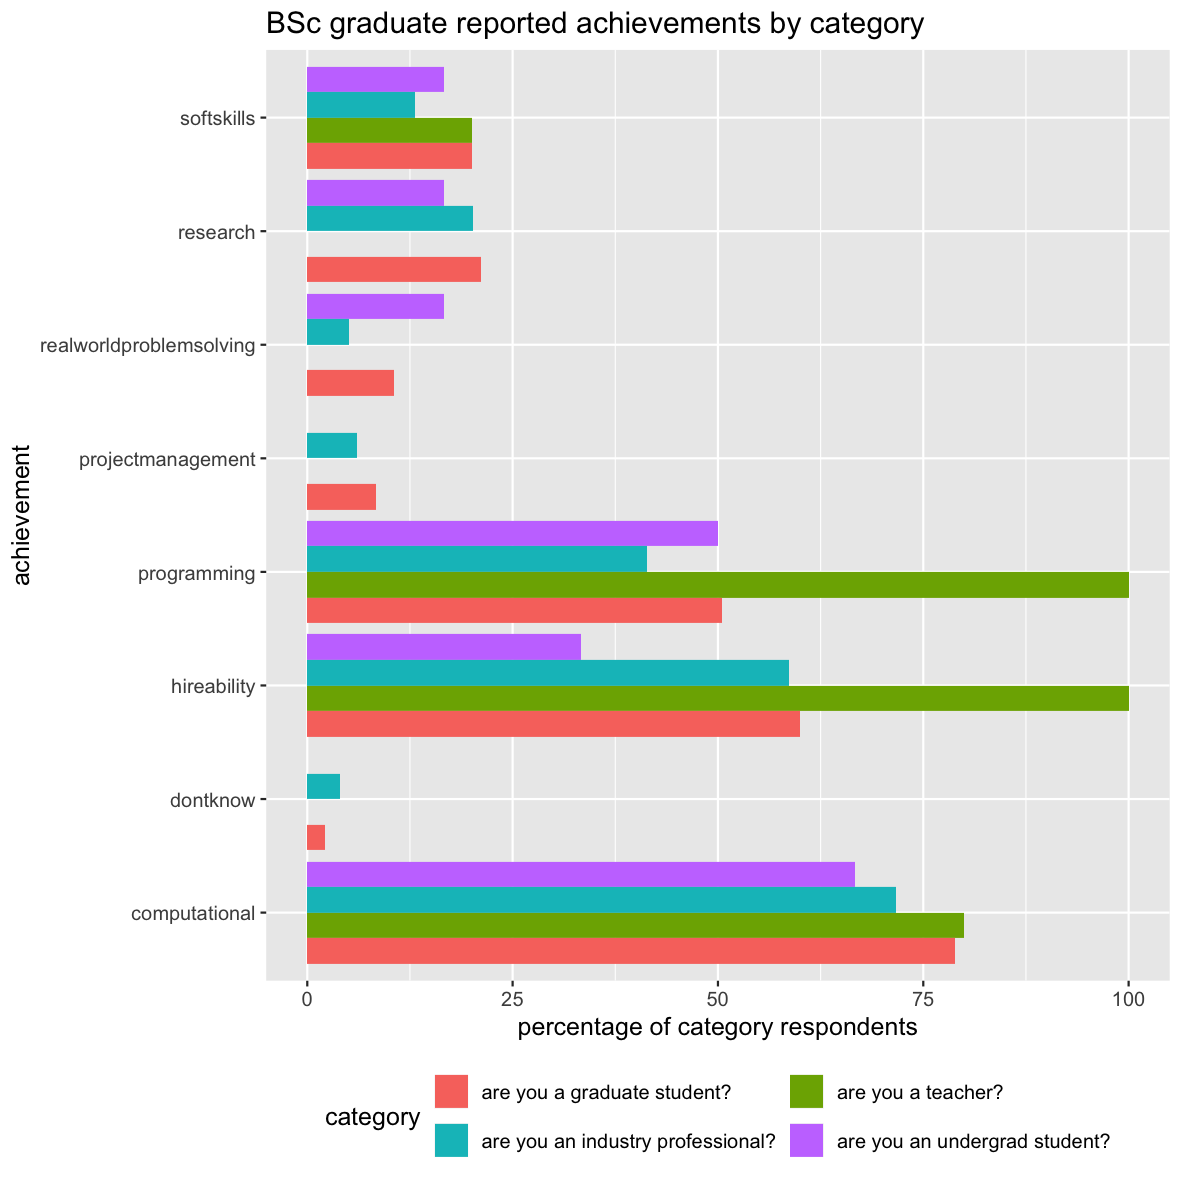
\includegraphics[scale=0.2]{../data-analysis/plots_output/BSc_graduate_reported_achievements_by_category.png}
 \caption{Currently, what do you think an UNDERGRADUATE student in CS or SE achieves, when he/she graduates?}~\label{fig:figure1}
\end{figure}

Figure \ref{fig:figure1} shows that most of our respondents, regardless of their category, think that a BS graduate achieves the so-called \textit{computational thinking}, and, secondarily, a certain chance of getting hired and some programming skills. Here, we can actually see a bit of contrast between two categories: the teachers, and the industry professionals. The former group think that programming is something a BS graduate definitely acquires; the latter, being the ones that actually employ such skills, are far more reluctant to say that you get this skill in university.

Regarding the would-like skills, there are not great surprises; it seems that the most interesting selected items, that aren't achieved at university, are real-world problem solving, soft skills, and project management (Fig. \ref{fig:figure2}). Undergrads especially did not vote for this latest skills, however, improvement on chances of getting hired is one of this category's would-like achievements from academic educations.

One surprise comes from programming skills for undergrads. It's not marked as a clear achievement by most respondent, and \textbf{neither it is marked as a desiderata}. How should somebody hone his programming skills? On the other hand, it seems that programming skill is mostly achieved by post-graduate level students and is not selected as a high demand for would-like achievements. 

The other surprise comes from research skills. Teachers don't think it's something that is taught, and neither that should be taught. Possibly, that's left to graduate education?

\begin{figure}
 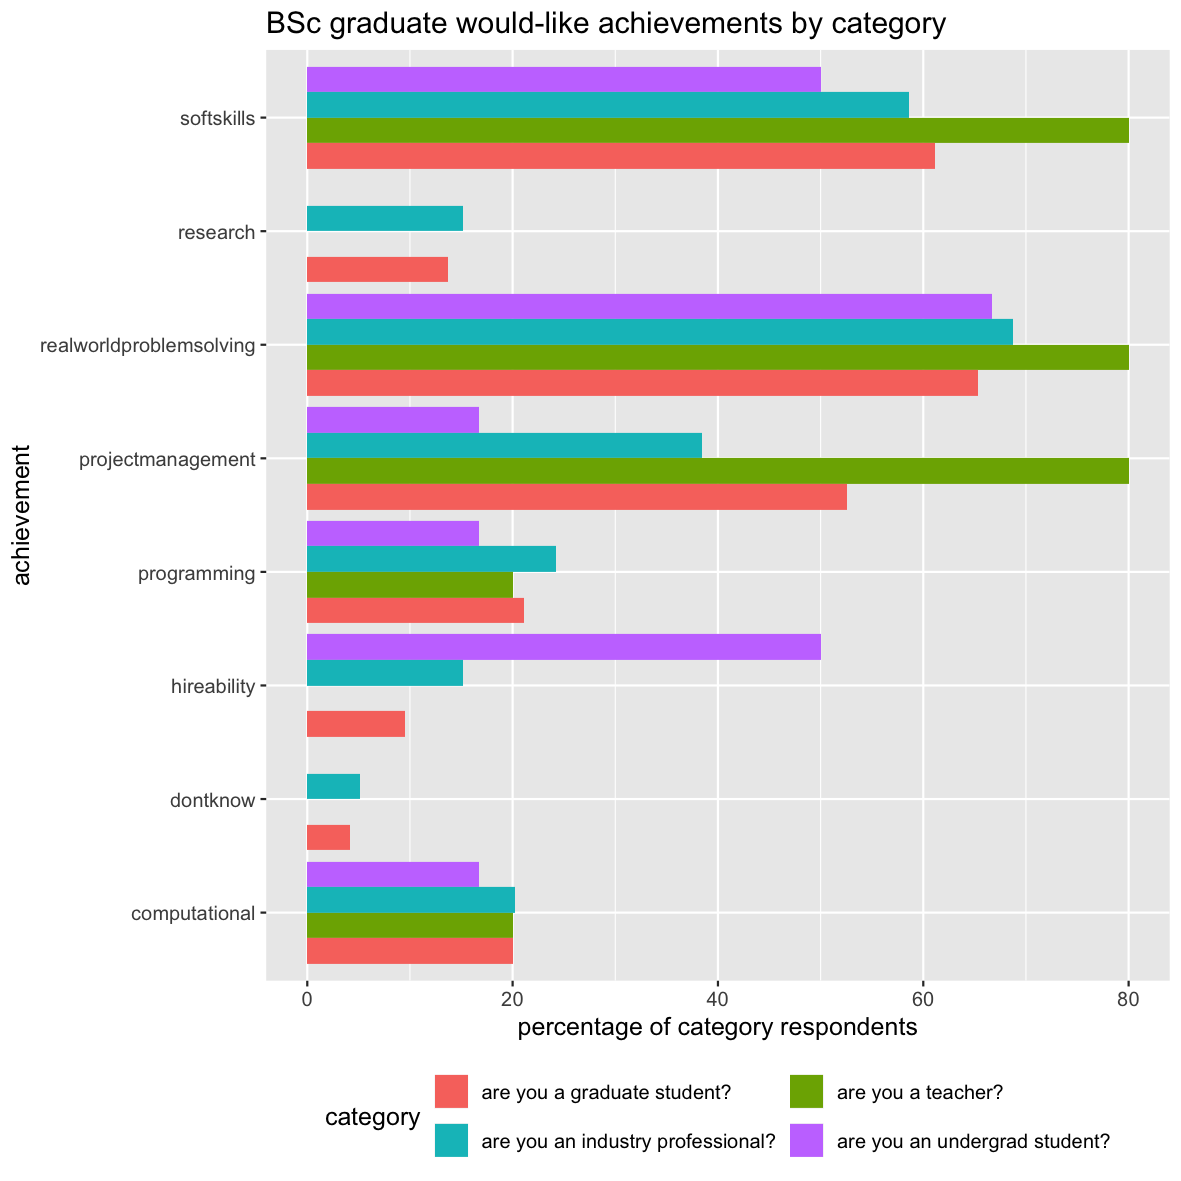
\includegraphics[scale=0.2]{../data-analysis/plots_output/BSc_graduate_would-like_achievements_by_category.png}
  \caption{Are there any skills, that you think an UNDERGRADUATE student would need to learn at university, where it is not taught by universities, and are essential in working industry?}~\label{fig:figure2}
\end{figure}

Next, we investigated the opinions about graduate education (Fig.  \ref{fig:figure3} \& Fig.  \ref{fig:figure4}) . It appears to be a partial solution for some parts of undergrad education, but not completely. Most people \textit{but industry professionals and graduate-level students} would agree that MS education improves your programming skills; since industry professionals are actually the most qualified at such opinion, it's not really encouraging, since they estimate MS graduate abilities on par with BS graduate abilities. On the other hand, teachers and undergraduate students categories (> 75\%) selected this skill as an achievement after MS graduation.

\begin{figure}
 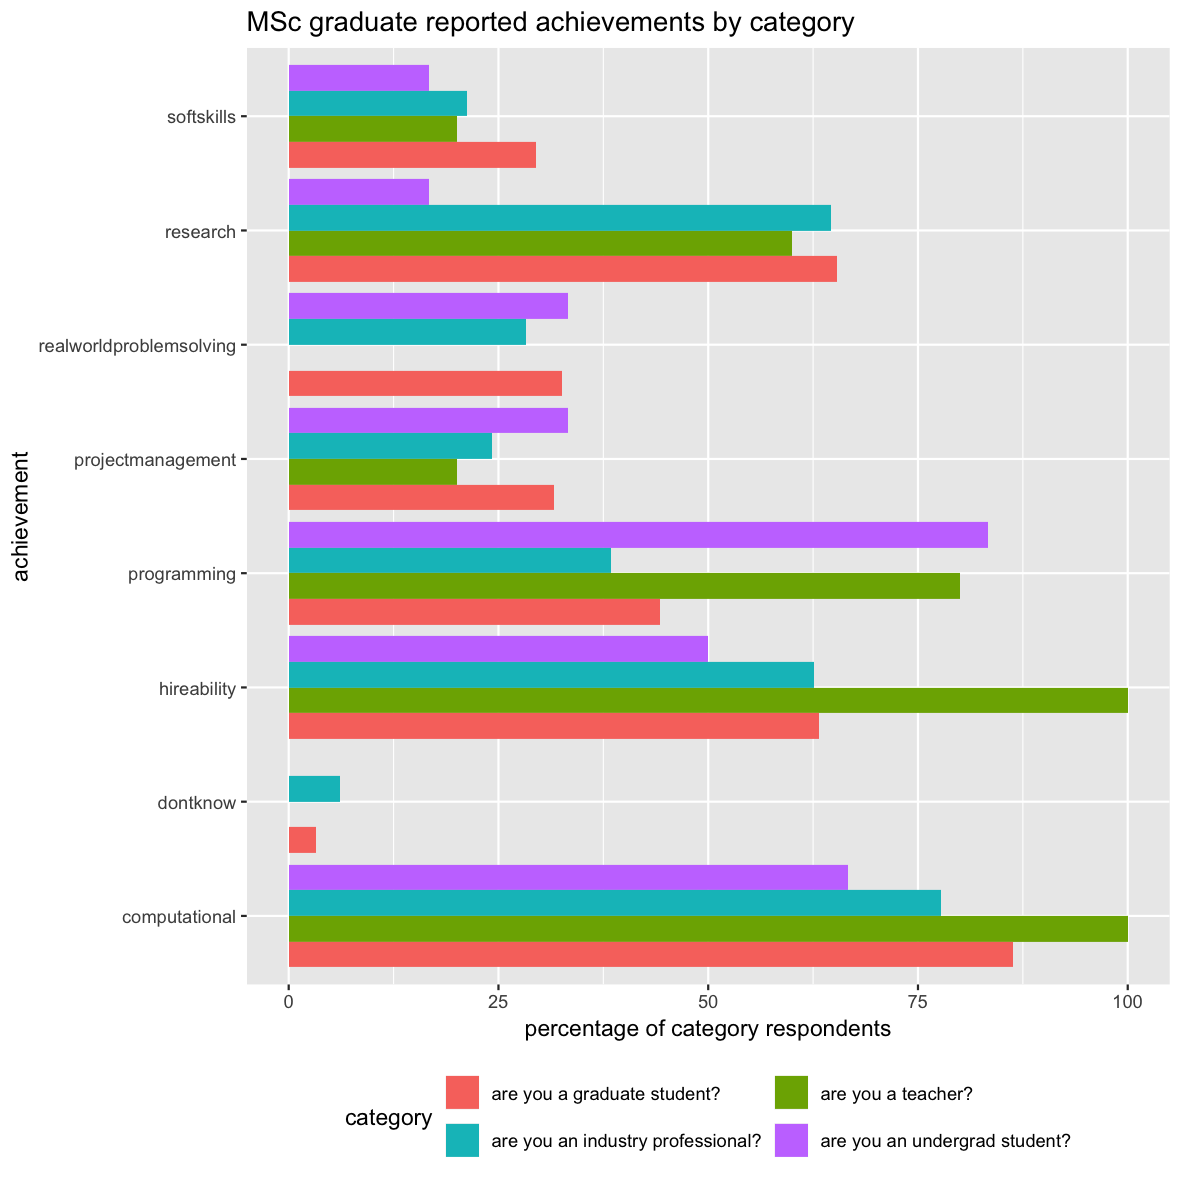
\includegraphics[scale=0.2]{../data-analysis/plots_output/MSc_graduate_reported_achievements_by_category.png}
  \caption{Currently, what do you think an GRADUATE student (MS program) in CS or SE achieves, when he/she graduates?}~\label{fig:figure3}
\end{figure}

We see better results for research: a reasonable amount of respondents think that graduate education is the  stage at which research skills are taught.

But real-word problem solving is still an open problem, even after a MS degree; and soft skills, along project management, could fare much better; there seem to be a large amount of teachers that agree on the fact that MS graduates would need more skills that can be applied directly in the real world.

\begin{figure}
 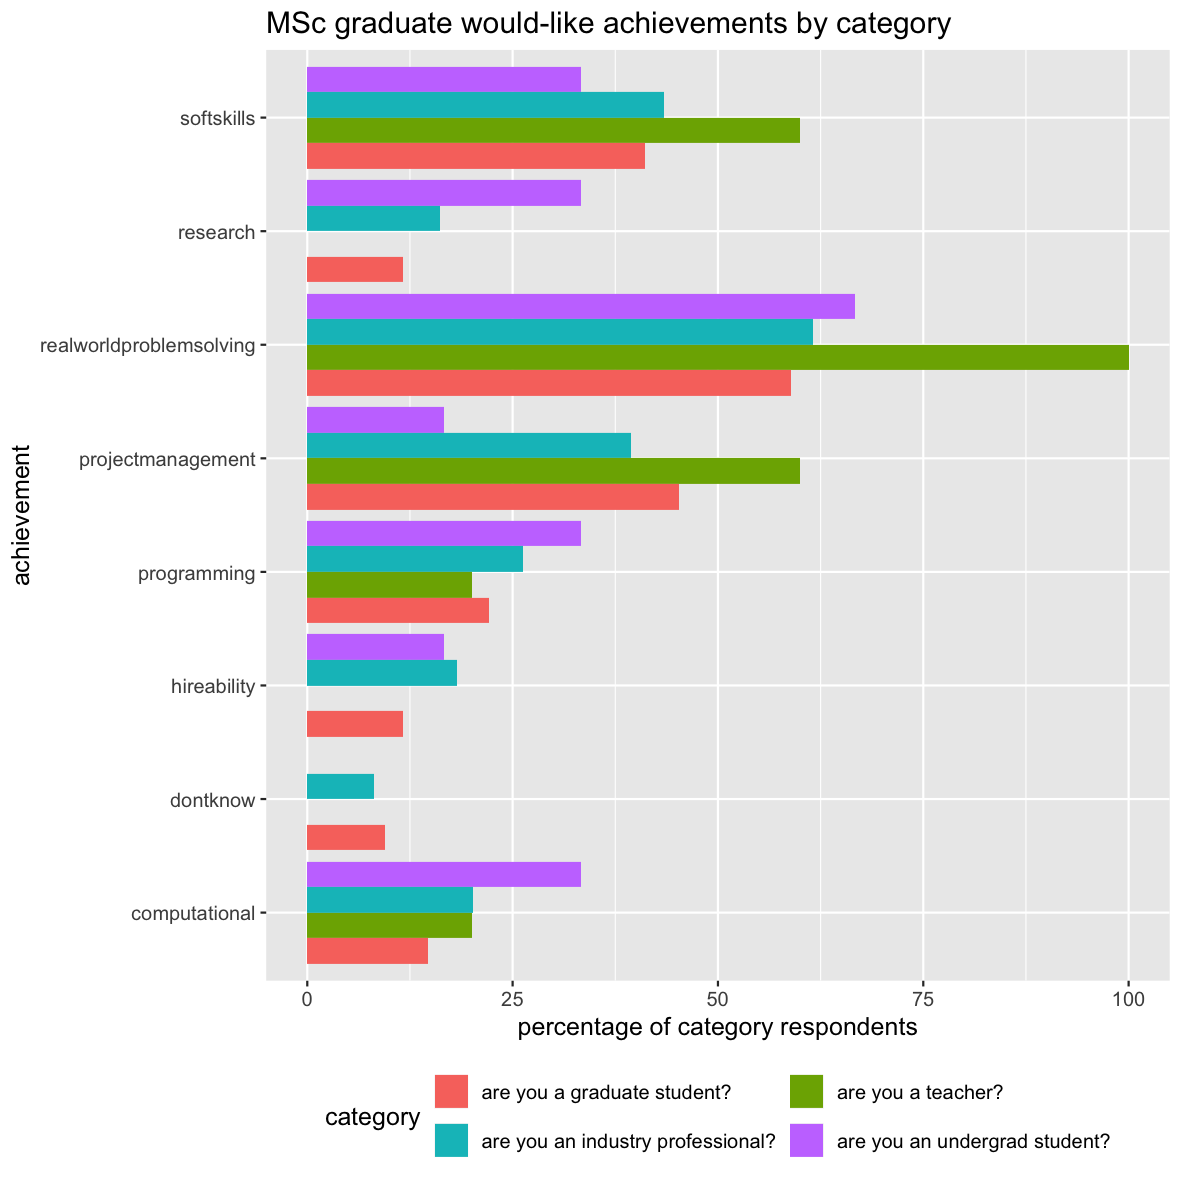
\includegraphics[scale=0.2]{../data-analysis/plots_output/MSc_graduate_would-like_achievements_by_category.png}
  \caption{Are there any skills, that you think an GRADUATE student (MS program) would need to learn at university, where it is not taught by universities, and are essential in working industry?}~\label{fig:figure4}
\end{figure}

Generally, we can see more traces of this belief in another answer (Fig. \ref{fig:figure5}). Only a few undergrads (12.5\%) hope that, at the end of their four-year studies, they'll have a high chance to enter the workforce and just have a great career (Fig. \ref{fig:figure5}). Other categories mostly believe that an apprenticeship phase will be mandatory for everybody - in this phase, most probably our graduates will learn about \textbf{soft skills, project management, real-world problem solving, and actual programming}.

\begin{figure}
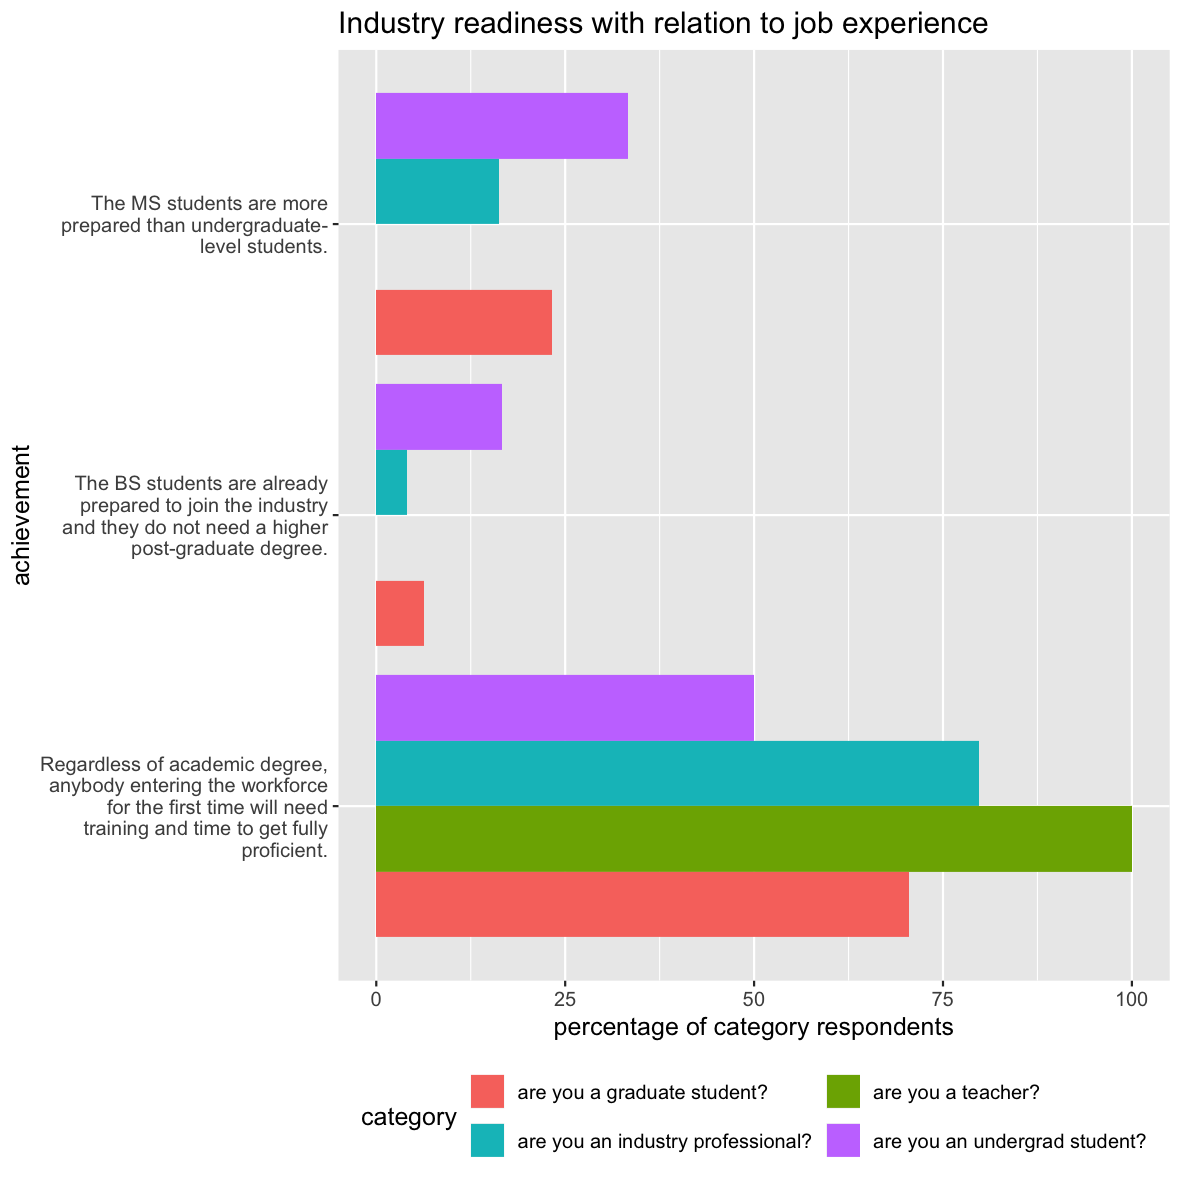
\includegraphics[scale=0.2]{../data-analysis/plots_output/Industry_readiness_with_relation_to_job_experience.png}
 \caption{In general, which statement, in your opinion, is more accurate? (if we assume that below groups have no previous job experience)}~\label{fig:figure5}
\end{figure}

This idea is reinforced as we asked our respondents to compare experienced and unexperienced candidates with and without degrees (Fig. \ref{fig:figure6} \& Fig. \ref{fig:figure7}). As we can see, a large majority (between 75\% to 80\%) thinks that experience matters a lot. Interestingly, teachers seem that experience is even more important, probably acknowledging the industry-school expectation gap and our supposed misalignment.

\begin{figure}
 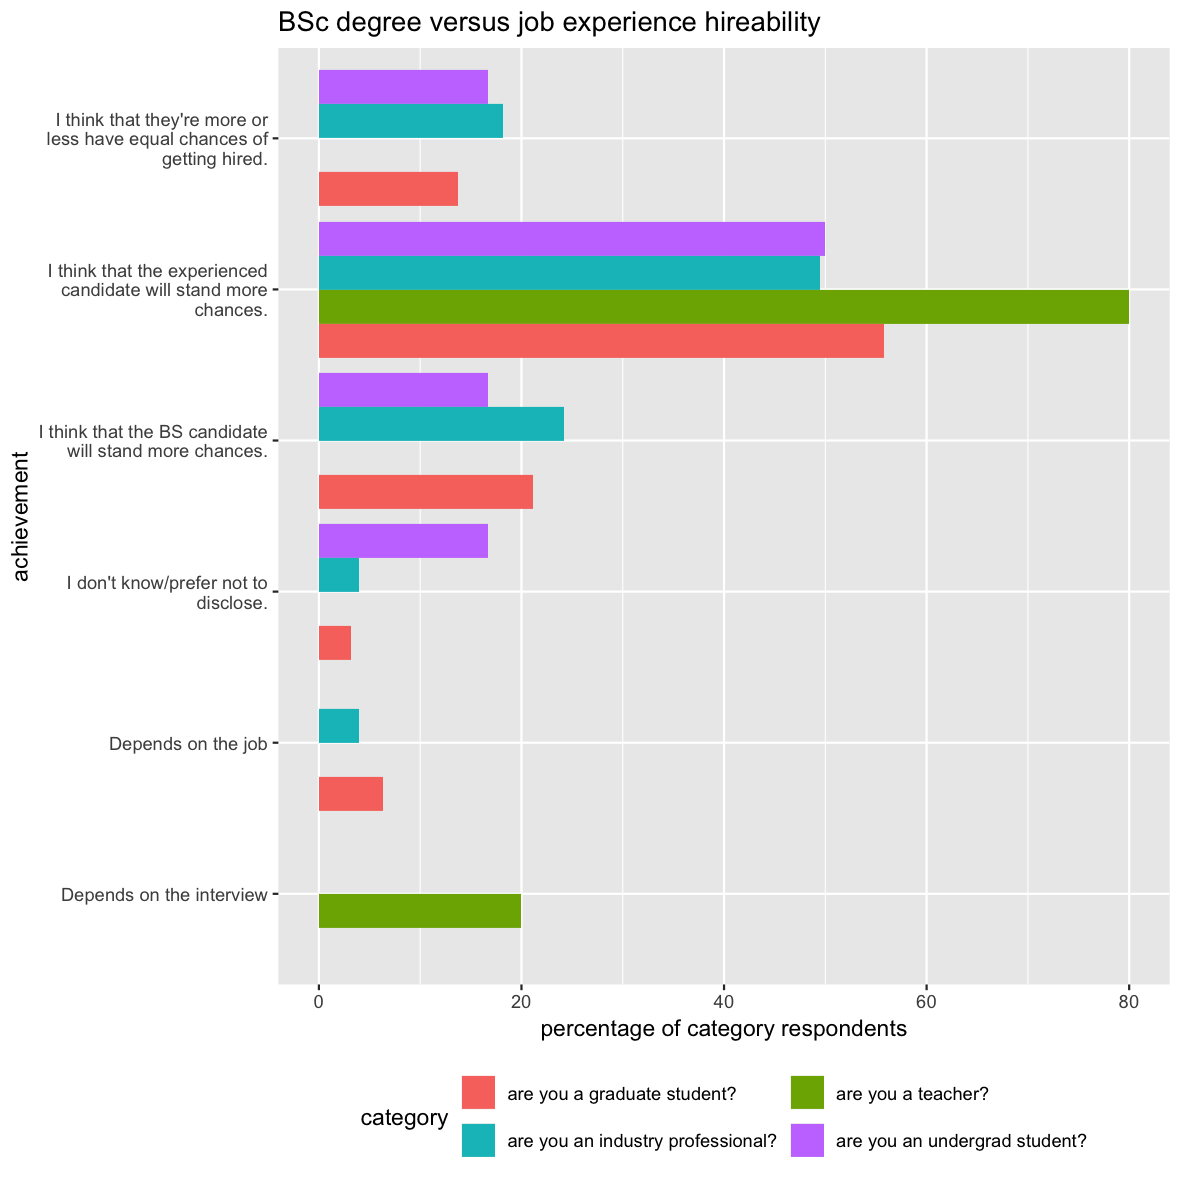
\includegraphics[scale=0.2]{../data-analysis/plots_output/BSc_degree_versus_job_experience_hireability.png}
  \caption{Consider two candidates for a same job. One holds a 4-year BS degree and has no job experience. The other has no degree, but has 4 years of job experience in a similar role. What do you think about the candidates' chance of being hired?}~\label{fig:figure6} %TODO: verify this graph: it seems a bit off, some categories seem to sum to more than 100%
\end{figure}

\begin{figure}
 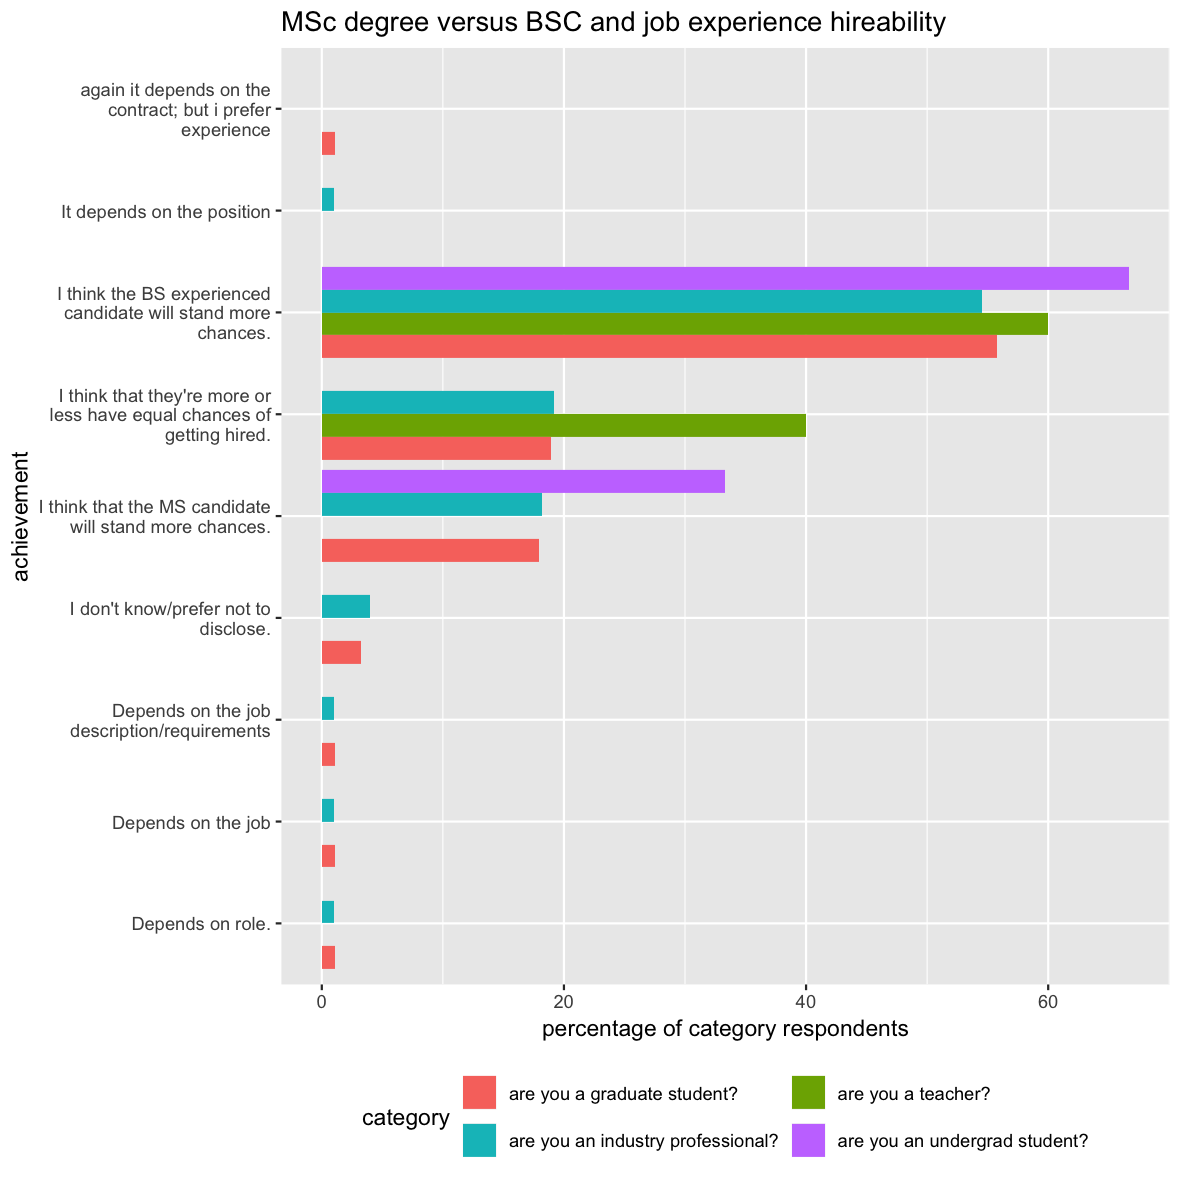
\includegraphics[scale=0.2]{../data-analysis/plots_output/MSc_degree_versus_BSC_and_job_experience_hireability.png}
  \caption{Consider two candidates for the same job. One holds a relevant MS degree and no job experience. The other has a BS and 2-years of relevant job experience. What do you think about the candidates' chance of being hired?}~\label{fig:figure7}
\end{figure}

One last interesting result explains the job proficiency in short-term and long-term for both BS and MS graduates (Fig \ref{fig:figure8} to Fig. \ref{fig:figure11}).

\begin{figure}
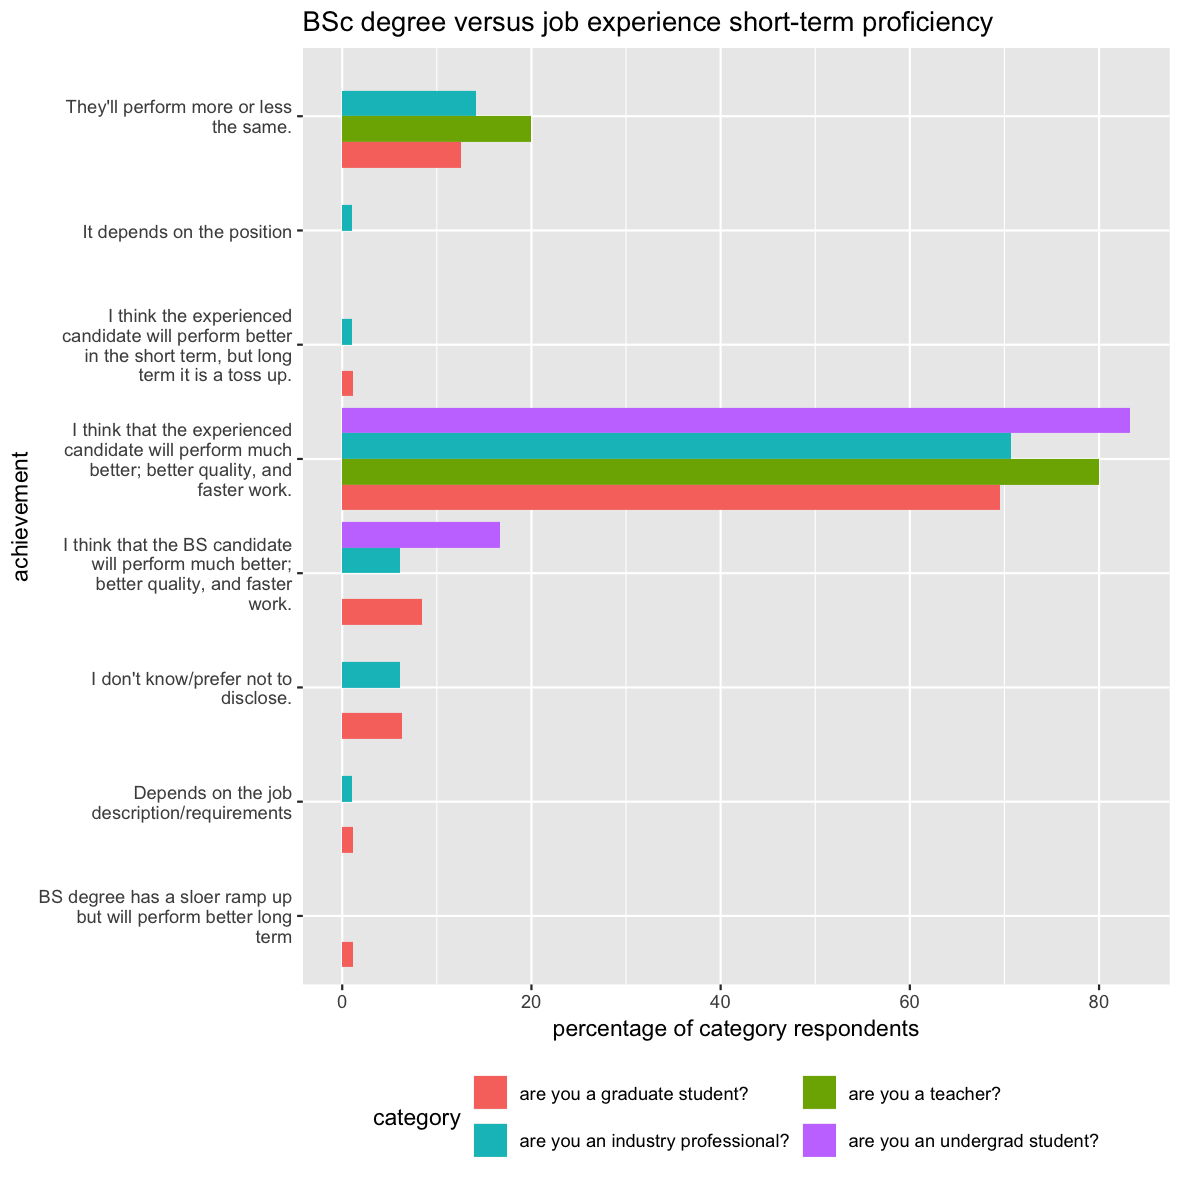
\includegraphics[scale=0.2]{../data-analysis/plots_output/BSc_degree_versus_job_experience_short-term_proficiency.png}
 \caption{Consider two fresh hires for the same position at the same company. One holds a 4-year BS degree and no job experience. The other has no degree, but has 4 years of job experience in a similar role. What do you think about the candidates' skills and performance RIGHT AFTER BEING HIRED?}~\label{fig:figure8}
\end{figure}

\begin{figure}
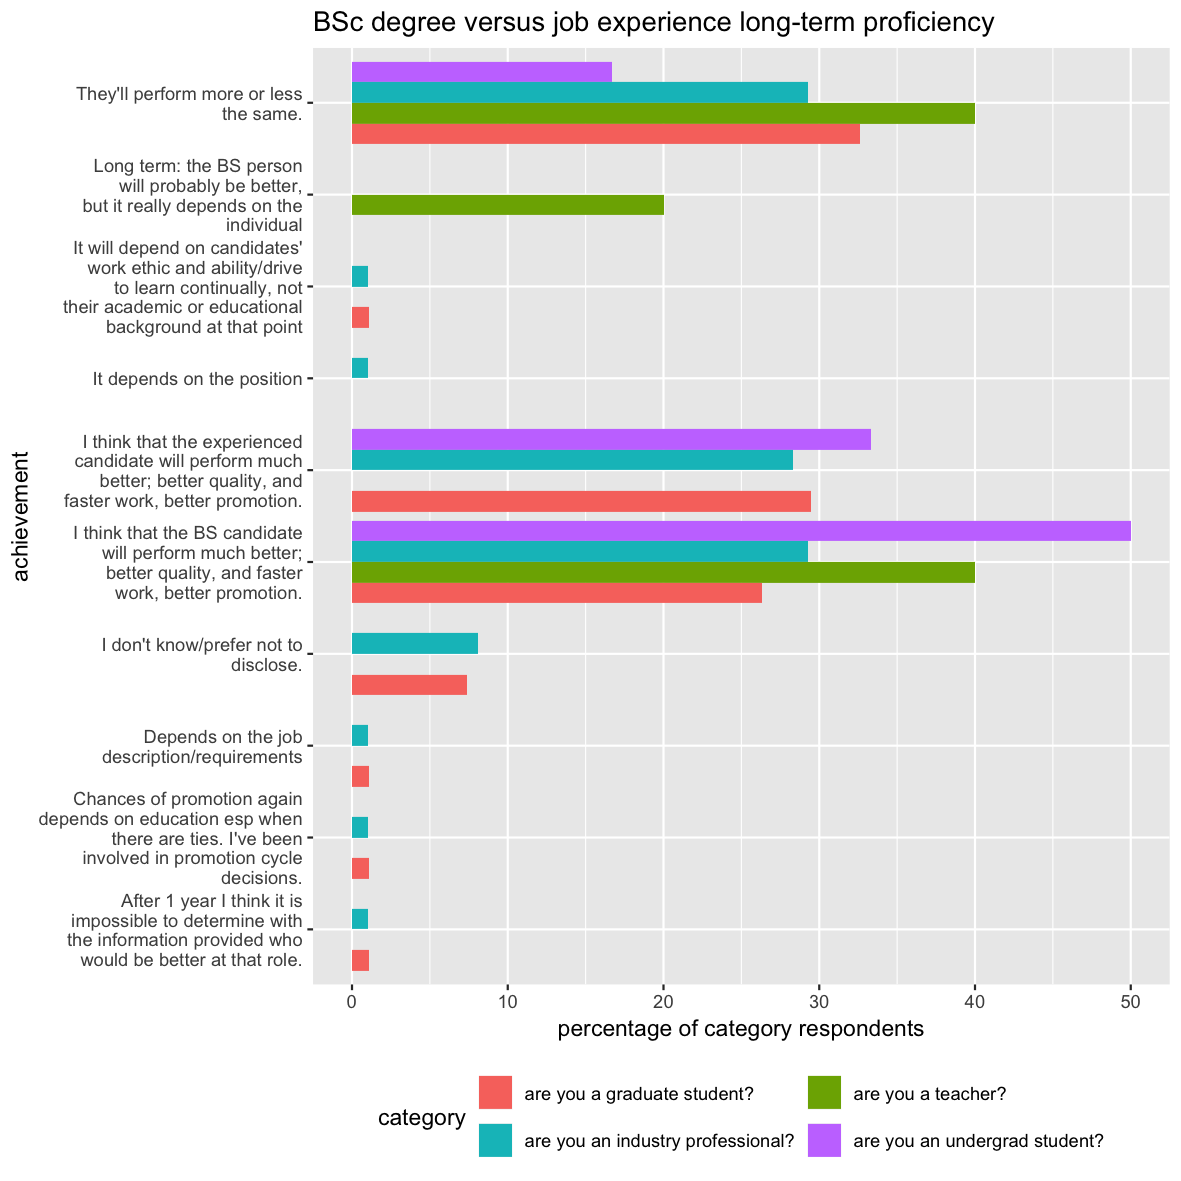
\includegraphics[scale=0.2]{../data-analysis/plots_output/BSc_degree_versus_job_experience_long-term_proficiency.png}
 \caption{Consider two fresh hires for the same position at the same company. One holds a 4-year BS degree and no job experience. The other has no degree, but has 4 years of job experience in a similar role. They work at the company, in the same role, for one year. What do you think about the candidates' skills and career at that time (after 1 year)?}~\label{fig:figure9}
\end{figure}

\begin{figure}
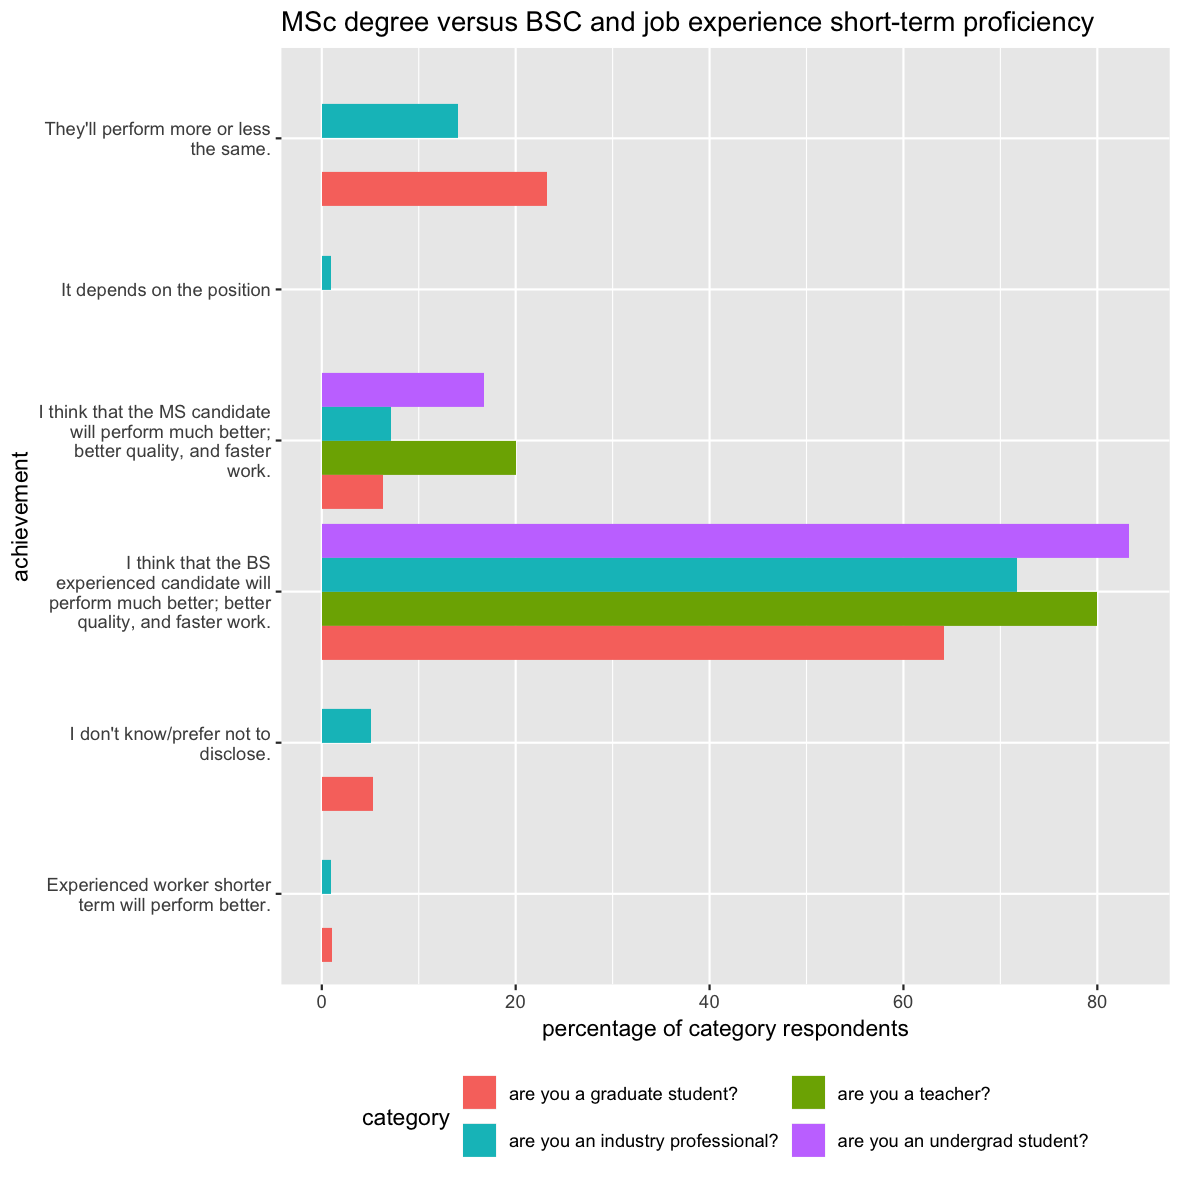
\includegraphics[scale=0.2]{../data-analysis/plots_output/MSc_degree_versus_BSC_and_job_experience_short-term_proficiency.png}
 \caption{Consider two fresh hires for the same position at the same company. One holds a relevant MS degree and no job experience. The other has a BS degree, and a couple of years of experience in a similar role. What do you think about the candidates' skills and performance RIGHT AFTER BEING HIRED?}~\label{fig:figure10}
\end{figure}

\begin{figure}
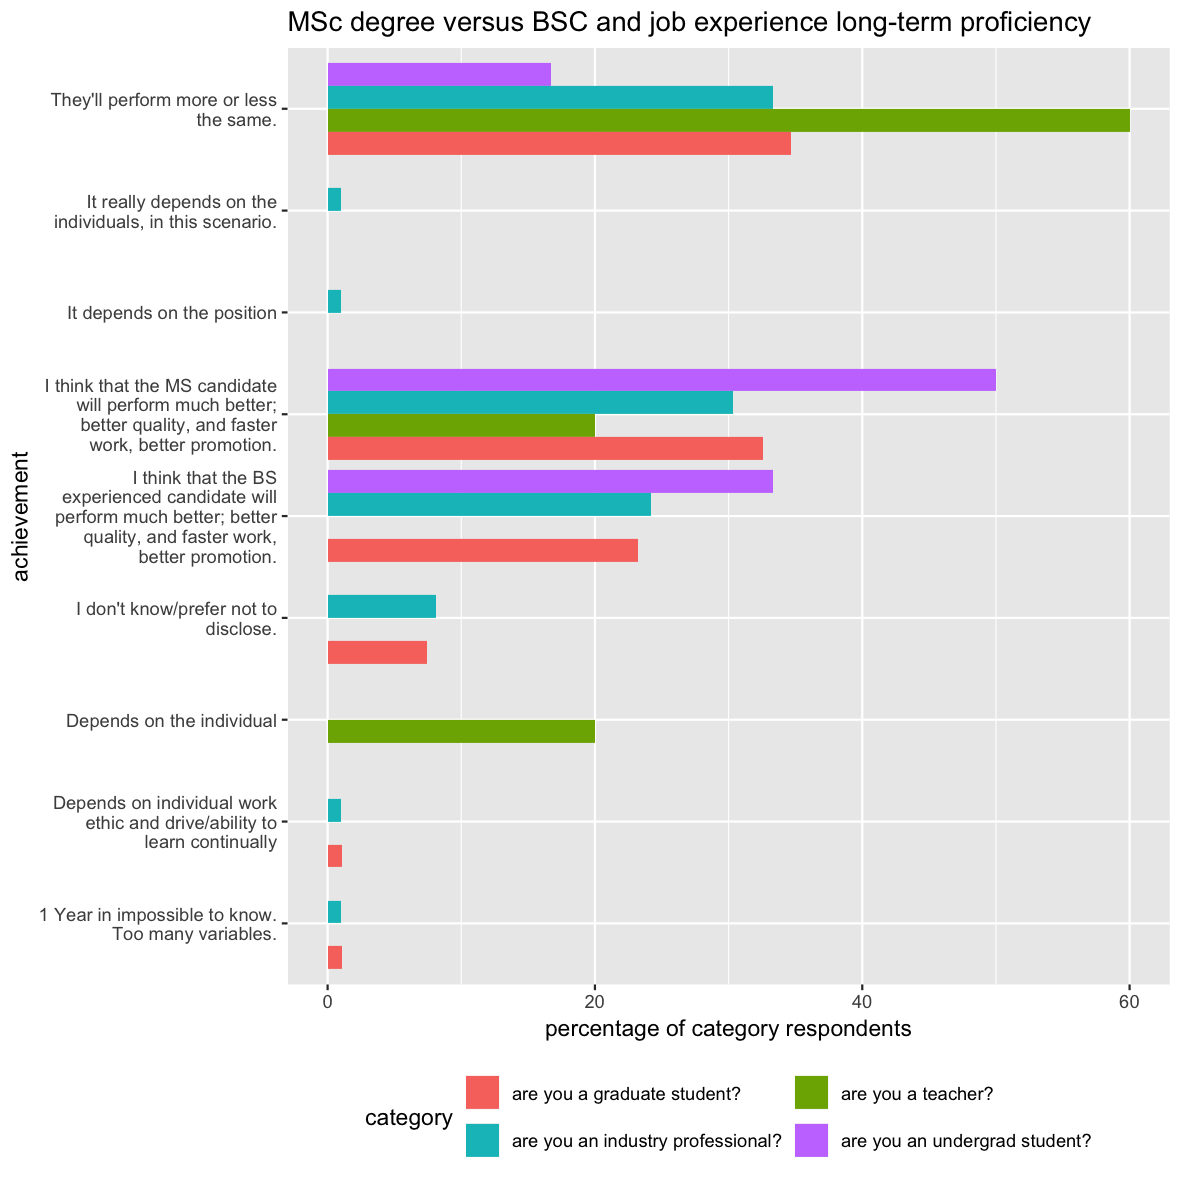
\includegraphics[scale=0.2]{../data-analysis/plots_output/MSc_degree_versus_BSC_and_job_experience_long-term_proficiency.png}
 \caption{Consider two fresh hires for the same role at the same company. One holds an MS degree and no job experience. The other has a BS degree, and 2 years of job experience in a similar role. They work at the company, in the same role, for one year. What do you think about the candidates' skills and career at that time (after 1 year)?}~\label{fig:figure11}
\end{figure}

\begin{figure*}
  \centering
  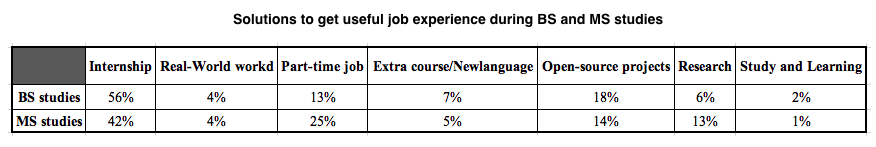
\includegraphics[width=1.75\columnwidth]{../data-analysis/plots_output/Solutions_to_gain_useful_job_experience.png}
  \caption{In your opinion, how can students gain useful work experience during their BS and/or MS studies, if any?}~\label{fig:figure12}
\end{figure*}

\begin{figure}
  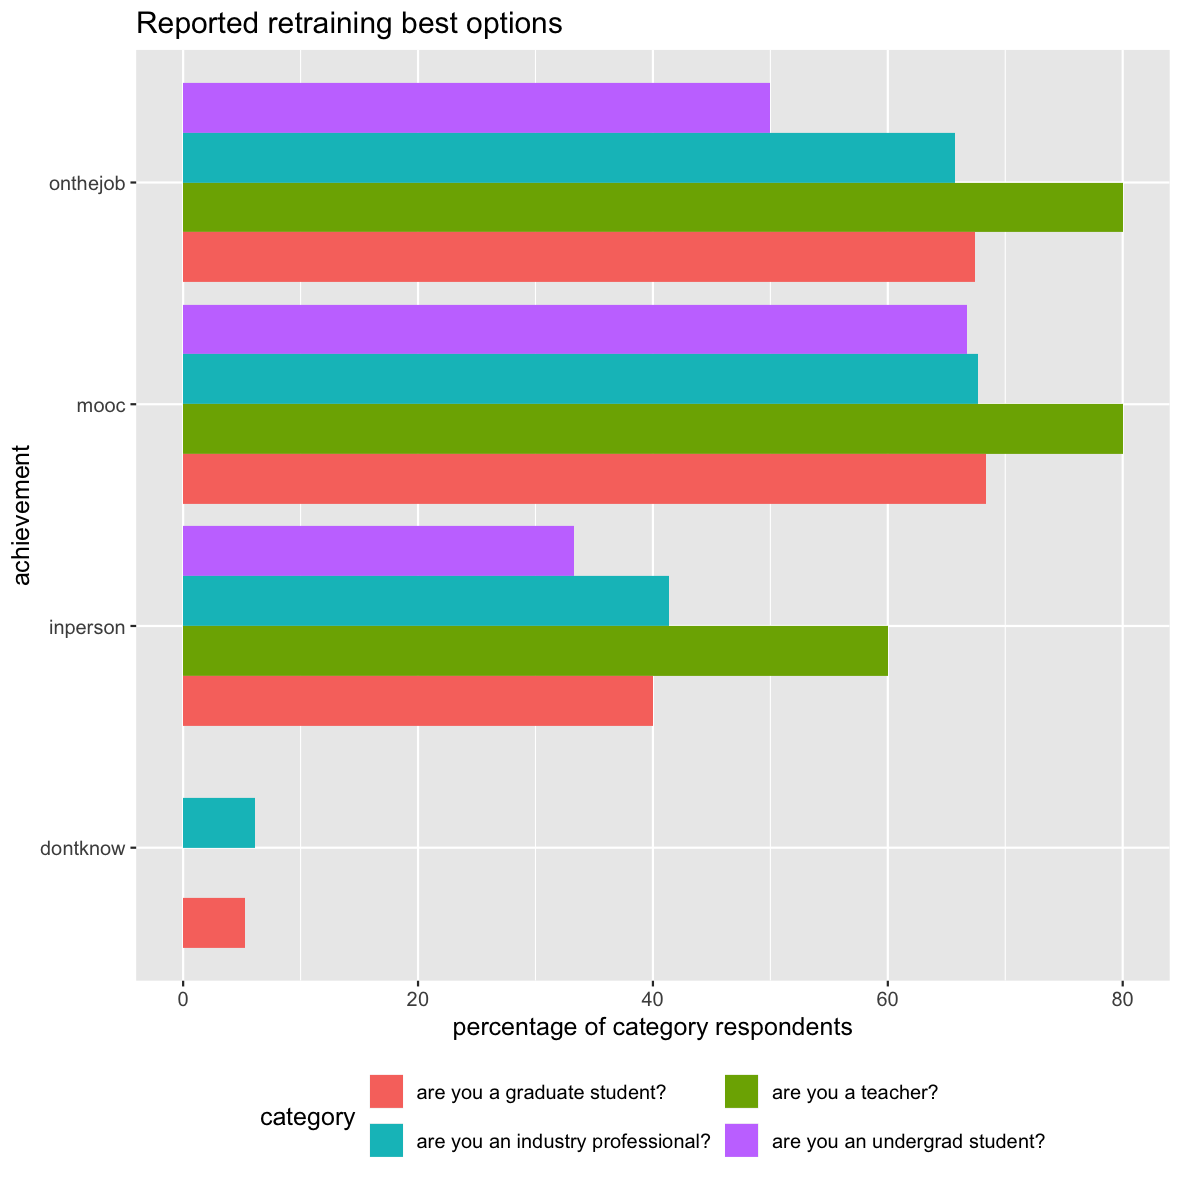
\includegraphics[scale=0.2]{../data-analysis/plots_output/Reported_retraining_best_options.png}
  \caption{In your opinion, what could be valid alternatives to a Master's degree for a professional in need of retraining?}~\label{fig:figure13}
\end{figure}

Here, we can explain two things:
\begin{itemize}
	\item In the short term, experience is more effective than a degree.
	\item In the long term, a degree doesn't necessarily mean a better worker.	
\end{itemize}

While the first statement may be a bit expected, we think that the second is clearly a novelty; even teachers don't acknowledge a clear advantage for graduates at doing their job. This is quite a clear image of the misalignment: there seems to be at least a slight indication that people in the academy don't really think that a lot of the topics they teach are \textit{that} aligned with modern industry requirements, neither in short-term nor long-term proficiency.

We have seen quite scattered responses about the impact of GPAs and top schools, and we don't think we can draw big conclusions about those topics.

In the next step, we collected data about possible solutions and suggestions on how the students in both levels can gain useful work experience during their studies. We found that most frequent answers are as internships, real-world work, part-time jobs, extra courses or learning new languages, open-source projects, research, and studying (Fig. \ref{fig:figure12}). As it shows in the table, the majority of the participants pointed out "internships" as the most effective practice for that. The next two major suggestions are part-time job and open-source projects. It is interesting that the part-time job is selected doubled the time for MS studies compared to BS studies. Another item to point out is that 13\% of the respondents think that research play an important role in MS studies to gain useful work experience. However, only 6\% recommend research as an option to be better prepared for job industry.

In Fig. \ref{fig:figure13}, we looked at valid alternatives to MS education for a professional in need of retraining. As we expected, the Massive Open Online Course (MOOC) and, certainly, on-site job training received the highest percentage among all the categories. The "in-person learning" received less than 40\% of responses from all categories except teachers and professors. About 60\% of professors think that in-person studies can be a convincing option for MS studies. Another interesting item is to compare undergraduate-level students responses regarding on-site job training and MOOC options. It shows that there is about 20\% increase in choosing MOOC compared to on-site job training. This shows the high demand from undergraduate students to attend high-level online graduate programs and substitute this option with other in-person training and studies.

\section{Limitations}
 We think our research has several limitations.

First: we didn't get as many responses as we would like. We got about half the responses we were expecting.

Second: our categories are quite polarized. We've got a lot of industry professionals and graduate students, but we lack teachers and undergraduate students. Surely ,those few undergrads and teachers' opinion has a disproportionate effect in our analysis.

Third: most of our respondents come from the US. We don't think this research can have a worldwide validity, it's probably just one view of the problem.

Fourth: we had initially missed (an error while converting a document to Google Forms) a fundamental question in our survey (the category). Since we knew some of the respondents, we have inferred the categories for our analysis' sake for a small set of initial respondents (the survey was later amended).

\section{Conclusions}
About our two main hypotheses, we could say that:

For the first hypothesis, we could say that collected data \textit{partially supports} it. Undergrad programs aren't meant to teach project management, problem solving, or soft skills, while a lot of people would just love to see Bachelors graduate with such abilities; so, there's a misalignment between the intentions of the industry and of the researchers. Interestingly, most undergrad students seem fully aware of the situation.

Programming, on the contrary, seems a matter of teaching abilities. It seems that schools are unable to create good programmers. But then, most people just seem to think that apprenticeship and on-the-job training are not replaceable by pure education; maybe we should just accept that we're yet unable to abstract away that kind of learning from real-world experience, and we should scale down students (and employers!) expectations about new graduates: they won't be good programmers without an appropriate on-the-job training.

The graduate education part appears to be a bit more foggy. We supposed that graduate-level programs would better fill the school-industry gap, but we cannot say that this is the case. Most of the industry is not concerned with research, and most industry professionals don't see great programming skills in MS graduates. For sure, it's a beginning, it's something more than basic BS education; but, probably, spending the same amount of time on a real job would yield the same results about soft skills, real-world problem solving and project management.

\section{Possible Future Works}
We think it would be very interesting to replicate the experiment on a different scale, with slightly different premises. \textbf{Recruitment} seems to be the hardest part of our research; it would be interesting to partner with some large organizations (be it companies, conferences, universities) in order to push a (similar) survey to them.

Many people (in online forums where we had spread our survey as well) told us one interesting point about the "chances to get hired" section: the experience, or the degree, only matter up to a point in order to be \textit{hired}. It may matter in order \textit{to get an interview}: if we ever replicate this survey, it would be better to substitute "hireability" with "chances to land an interview".

It would be interesting to investigate the concept of good programmers, as well. Do bootcamps/MOOCs/other kind of programs produce better coders than university? Are they on par, but within a shorter timeframe? Could the university improve something?

It may be interesting to check if multiple categories (e.g. industry professionals that are MS students as well) have significantly different answers from "bare" categories; this was a bit outside the scope of our analysis because of time constraints and because of the polarization of our respondents, but could be quite useful.

It would be very useful to get more data from the academy. We haven't seen a clear indication for the purpose of the higher education programs; we may say that they appear a bit confused on whether it would like to focus on research, or it would like to help more the industry, or would just pursue knowledge for knowledge's sake - which could be a totally valid purpose!

\balance{}

\balance{}

% REFERENCES FORMAT
% References must be the same font size as other body text.
\bibliographystyle{SIGCHI-Reference-Format}
\bibliography{../bibliography.bib}

\end{document}

%%% Local Variables:
%%% mode: latex
%%% TeX-master: t
%%% End:
 